%%%%%%%%%%%%%%%%%%%%%%%%%%%%%%%%%%%%%%%%%per fare le conclusioni
\chapter*{Conclusioni}
%%%%%%%%%%%%%%%%%%%%%%%%%%%%%%%%%%%%%%%%%imposta l'intestazione di pagina
\rhead[\fancyplain{}{\bfseries
Conclusioni}]{\fancyplain{}{\bfseries\thepage}}
\lhead[\fancyplain{}{\bfseries\thepage}]{\fancyplain{}{\bfseries
Conclusioni}}
\addcontentsline{toc}{chapter}{Conclusioni}

Lo stato dell'arte al momento in cui si scrive \`e un'applicazione in grado di gestire eventi, commissioni da svolgere, spese condivise con la possibilità di usufruire di una chat di messaggistica istantanea.\\
Attraverso l'utilizzo del database Firebase ed i suoi servizi viene offerta una sincronizzazione in tempo reale dei dati con la possibilità di consultarli anche offline.\\
L'applicazione pur garantendo l'uso quotidiano delle funzionalità può essere ulteriormente migliorata, aggiungendo funzionalità, rendendola più stabile e riscriverla anche per la piattaforma iOS. Alcune idee in fase di sviluppo che verranno implementante sono le seguenti:
\begin{itemize}
  \item Chat di messaggistica istantanea anche fra i singoli componenti del gruppo
  \item Migliore flessibilità e funzionalità nella gestione degli eventi
  \item Nuovi informazioni inseribili all'interno di una spesa o commissione
  \item Permettere all'utente di partecipare a più di un gruppo contemporaneamente
  \item Scrivere l'applicazione per iOS utilizzando il linguaggio Swift
\end{itemize}
Attualmente il codice dell'applicazione è presente su Gitlab\footnote{http://gitlab.com/}, in una repository privata, non appena l'applicazione sarà considerata stabile e con le funzionalità desiderate, verrà resa pubblica.\\
L'applicazione è stata scritta utilizzando il linguaggio di programmazione Kotlin, a differenza del linguaggio Java solitamente utilizzato nello sviluppo di applicazioni mobili Android.\\ L'utilizzo di Kotlin come linguaggio per lo sviluppo dell'applicazione ha permesso di analizare i nuovi concetti introdotti dal linguaggio e porlo a confronto con Java. Il confronto effettuato fra Java e Kotlin è stato possibile poichè si aveva a disposizione sia una parte del progetto scritta inizialmente in Java, sia la parte del progetto corrispondente in Kotlin.
I risultati ricavabili dal confronto effettuato, sono stati significativi soprattutto per quanto riguarda le linee di codice, alcune funzionalità che in Java richiedevano 140 linee di codice in Kotlin la stessa logica veniva implementata in circa 80 linee.\\
L'utilizzo della memoria e la dimensione dell'APK finale invece rimanevano inviariati,

\begin{figure}[!hb]
  \centering
  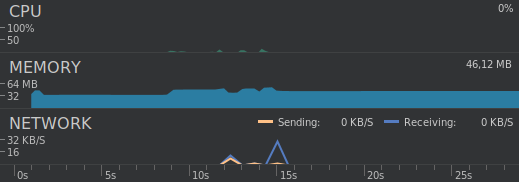
\includegraphics[width=0.8\textwidth]{immagini/app_java_memory_graph.png}
  \caption{Android Studio Memory Profile Java}\label{fig:Android Studio Memory Profile Java}
\end{figure}

\begin{figure}[!hb]
  \centering
  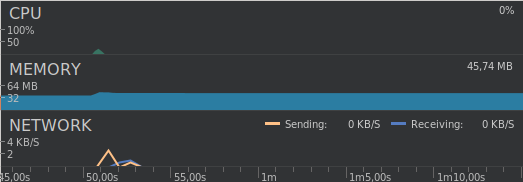
\includegraphics[width=0.8\textwidth]{immagini/app_kotlin_memory_graph.png}
  \caption{Android Studio Memory Profile Kotlin}\label{fig:Android Studio Memory Profile Kotlin }
\end{figure}
La tesi, il progetto, lo studio di Kotlin, e la realizzazione di un'infrastruttura server attraverso i servizi Firebase di Google, ha permesso di avere una visione globale della realizzazione di un applicazione in Kotlin, utilizzando tecnologie e tecniche di programmazione recenti.



\clearpage{\pagestyle{empty}\cleardoublepage}
